\documentclass[]{article}
\usepackage{lmodern}
\usepackage{amssymb,amsmath}
\usepackage{ifxetex,ifluatex}
\usepackage{fixltx2e} % provides \textsubscript
\ifnum 0\ifxetex 1\fi\ifluatex 1\fi=0 % if pdftex
  \usepackage[T1]{fontenc}
  \usepackage[utf8]{inputenc}
\else % if luatex or xelatex
  \ifxetex
    \usepackage{mathspec}
    \usepackage{xltxtra,xunicode}
  \else
    \usepackage{fontspec}
  \fi
  \defaultfontfeatures{Mapping=tex-text,Scale=MatchLowercase}
  \newcommand{\euro}{€}
\fi
% use upquote if available, for straight quotes in verbatim environments
\IfFileExists{upquote.sty}{\usepackage{upquote}}{}
% use microtype if available
\IfFileExists{microtype.sty}{%
\usepackage{microtype}
\UseMicrotypeSet[protrusion]{basicmath} % disable protrusion for tt fonts
}{}
\usepackage{biblatex}
\bibliography{addons/bib/myrefs.bib}
\usepackage{color}
\usepackage{fancyvrb}
\newcommand{\VerbBar}{|}
\newcommand{\VERB}{\Verb[commandchars=\\\{\}]}
\DefineVerbatimEnvironment{Highlighting}{Verbatim}{commandchars=\\\{\}}
% Add ',fontsize=\small' for more characters per line
\newenvironment{Shaded}{}{}
\newcommand{\KeywordTok}[1]{\textcolor[rgb]{0.00,0.44,0.13}{\textbf{{#1}}}}
\newcommand{\DataTypeTok}[1]{\textcolor[rgb]{0.56,0.13,0.00}{{#1}}}
\newcommand{\DecValTok}[1]{\textcolor[rgb]{0.25,0.63,0.44}{{#1}}}
\newcommand{\BaseNTok}[1]{\textcolor[rgb]{0.25,0.63,0.44}{{#1}}}
\newcommand{\FloatTok}[1]{\textcolor[rgb]{0.25,0.63,0.44}{{#1}}}
\newcommand{\CharTok}[1]{\textcolor[rgb]{0.25,0.44,0.63}{{#1}}}
\newcommand{\StringTok}[1]{\textcolor[rgb]{0.25,0.44,0.63}{{#1}}}
\newcommand{\CommentTok}[1]{\textcolor[rgb]{0.38,0.63,0.69}{\textit{{#1}}}}
\newcommand{\OtherTok}[1]{\textcolor[rgb]{0.00,0.44,0.13}{{#1}}}
\newcommand{\AlertTok}[1]{\textcolor[rgb]{1.00,0.00,0.00}{\textbf{{#1}}}}
\newcommand{\FunctionTok}[1]{\textcolor[rgb]{0.02,0.16,0.49}{{#1}}}
\newcommand{\RegionMarkerTok}[1]{{#1}}
\newcommand{\ErrorTok}[1]{\textcolor[rgb]{1.00,0.00,0.00}{\textbf{{#1}}}}
\newcommand{\NormalTok}[1]{{#1}}
\usepackage{graphicx}
\makeatletter
\def\maxwidth{\ifdim\Gin@nat@width>\linewidth\linewidth\else\Gin@nat@width\fi}
\def\maxheight{\ifdim\Gin@nat@height>\textheight\textheight\else\Gin@nat@height\fi}
\makeatother
% Scale images if necessary, so that they will not overflow the page
% margins by default, and it is still possible to overwrite the defaults
% using explicit options in \includegraphics[width, height, ...]{}
\setkeys{Gin}{width=\maxwidth,height=\maxheight,keepaspectratio}
\ifxetex
  \usepackage[setpagesize=false, % page size defined by xetex
              unicode=false, % unicode breaks when used with xetex
              xetex]{hyperref}
\else
  \usepackage[unicode=true]{hyperref}
\fi
\hypersetup{breaklinks=true,
            bookmarks=true,
            pdfauthor={任呈祥},
            pdftitle={测试标题},
            colorlinks=true,
            citecolor=blue,
            urlcolor=blue,
            linkcolor=magenta,
            pdfborder={0 0 0}}
\urlstyle{same}  % don't use monospace font for urls
\setlength{\parindent}{0pt}
\setlength{\parskip}{6pt plus 2pt minus 1pt}
\setlength{\emergencystretch}{3em}  % prevent overfull lines
\setcounter{secnumdepth}{0}

\title{测试标题}
\author{任呈祥}
\date{January 2014}

\usepackage[generate,ps2eps]{abc}

\begin{document}
\maketitle
\begin{abstract}
Lorem ipsum dolor sit amet, consectetur adipisicing elit, sed do eiusmod
tempor incididunt ut labore et dolore magna aliqua. Ut enimad minim
veniam, quis nostrud exercitation ullamco laboris nisi ut aliquip ex ea
commodo consequat. Duis aute irure dolor in reprehenderit in voluptate
velit esse cillum dolore eu fugiat nulla pariatur. Excepteur sint
occaecat cupidatat non proident, sunt in culpa qui officia deserunt
mollit anim id est laborum.
\end{abstract}

{
\hypersetup{linkcolor=black}
\setcounter{tocdepth}{3}
\tableofcontents
}
\section{Introduction}\label{introduction}

Lorem ipsum dolor sit amet, consectetur adipisicing elit, sed do eiusmod
tempor incididunt ut labore et dolore magna aliqua
\autocite{menni2002topological}. Notice that citation there
\autocite{Hu1984bourbaki}. Ut enimad minim veniam, quis nostrud
exercitation ullamco laboris nisi ut aliquip ex ea commodo consequat.

\section{Theory}\label{theory}

Lorem ipsum dolor sit amet, consectetur adipisicing elit, sed do eiusmod
tempor incididunt ut labore et dolore magna aliqua. Ut enimad minim
veniam, quis nostrud exercitation ullamco laboris nisi ut aliquip ex ea
commodo consequat. Lorem ipsum dolor sit amet, consectetur adipisicing
elit, sed do eiusmod tempor incididunt ut labore et dolore magna aliqua.
Ut enimad minim veniam, quis nostrud exercitation ullamco laboris nisi
ut aliquip ex ea commodo consequat. Duis aute irure dolor in
reprehenderit in voluptate velit esse cillum dolore eu fugiat nulla
pariatur. Excepteur sint occaecat cupidatat non proident, sunt in culpa
qui officia deserunt mollit anim id est laborum. Lorem ipsum dolor sit
amet, consectetur adipisicing elit, sed do eiusmod tempor incididunt ut
labore et dolore magna aliqua. Ut enimad minim veniam, quis nostrud
exercitation ullamco laboris nisi ut aliquip ex ea commodo consequat.
Duis aute irure dolor in reprehenderit in voluptate velit esse cillum
dolore eu fugiat nulla pariatur. Excepteur sint occaecat cupidatat non
proident, sunt in culpa qui officia deserunt mollit anim id est laborum.

\section{Conclusion}\label{conclusion}

Right now, your options for formatting bibliographies using Pandoc are
to offload the work to biblatex (or natbib), or have pandoc handle
everything via \texttt{citeproc} and CSL files. The latter way is
simpler and cleaner, especially if we want to preserve the ability to
easily generate both HTML and LaTeX/PDF outputs. You have to do two
things. First, explicitly specify the ``References'' header. Second,
pandoc does not (yet) support some standard layout options for
bibliography entries---it will treat each entry like a regular
paragraph, when we want the first lines of each bibliography entry to
have no indentation, with subsequent lines (if any) to hang in from the
margin. The LaTeX commands below the ``References'' header accomplish
this . The LaTeX commands are ignored when HTML is produced, and do not
show up in the output file.

\section{References}\label{references}

\setlength{\parindent}{-0.2in} \setlength{\leftskip}{0.2in}
\setlength{\parskip}{8pt} \vspace*{-0.2in} \noindent

Use this

\begin{abc}
X:7
T:Qui Tolis (Trio)
C:André Raison
M:3/4
L:1/4
Q:1/4=92
%%staves {(Pos1 Pos2) Trompette}   
K:F
%  
V:Pos1
%%MIDI program 78
"Positif"x3  |x3    |c'>ba|Pga/g/f|:g2a  |ba2    |g2c- |c2P=B  |c>de  |fga    |
V:Pos2
%%MIDI program 78
        Mf>ed|cd/c/B|PA2d |ef/e/d |:e2f  |ef2    |c>BA |GA/G/F |E>FG  |ABc-   |
V:Trompette
%%MIDI program 56
"Trompette"z3|z3    |z3   |z3     |:Mc>BA|PGA/G/F|PE>EF|PEF/E/D|C>CPB,|A,G,F,-|
\end{abc}

to get

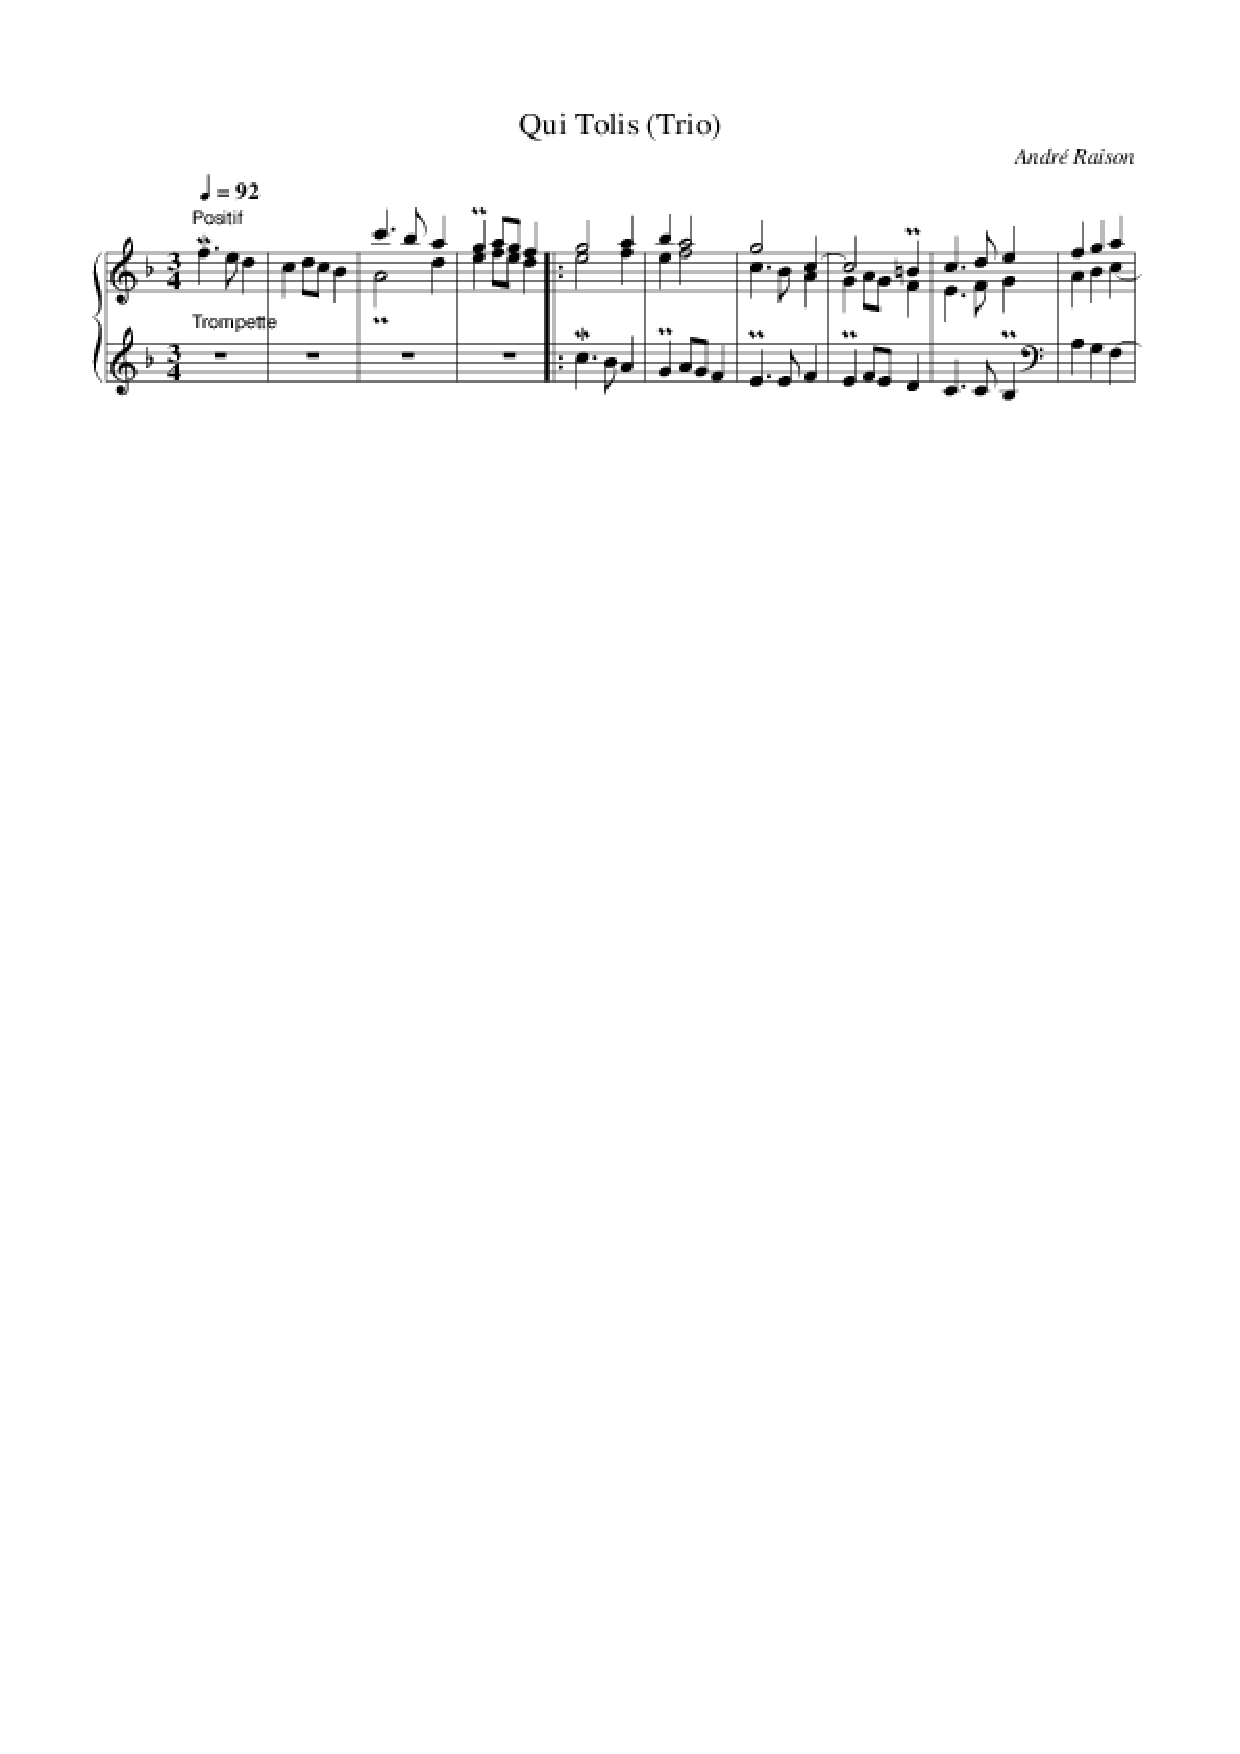
\includegraphics{../abc-images/d0fafff6e3eb537341f5d5eea7c29e2bc41ccc38.pdf}

lambda 2:

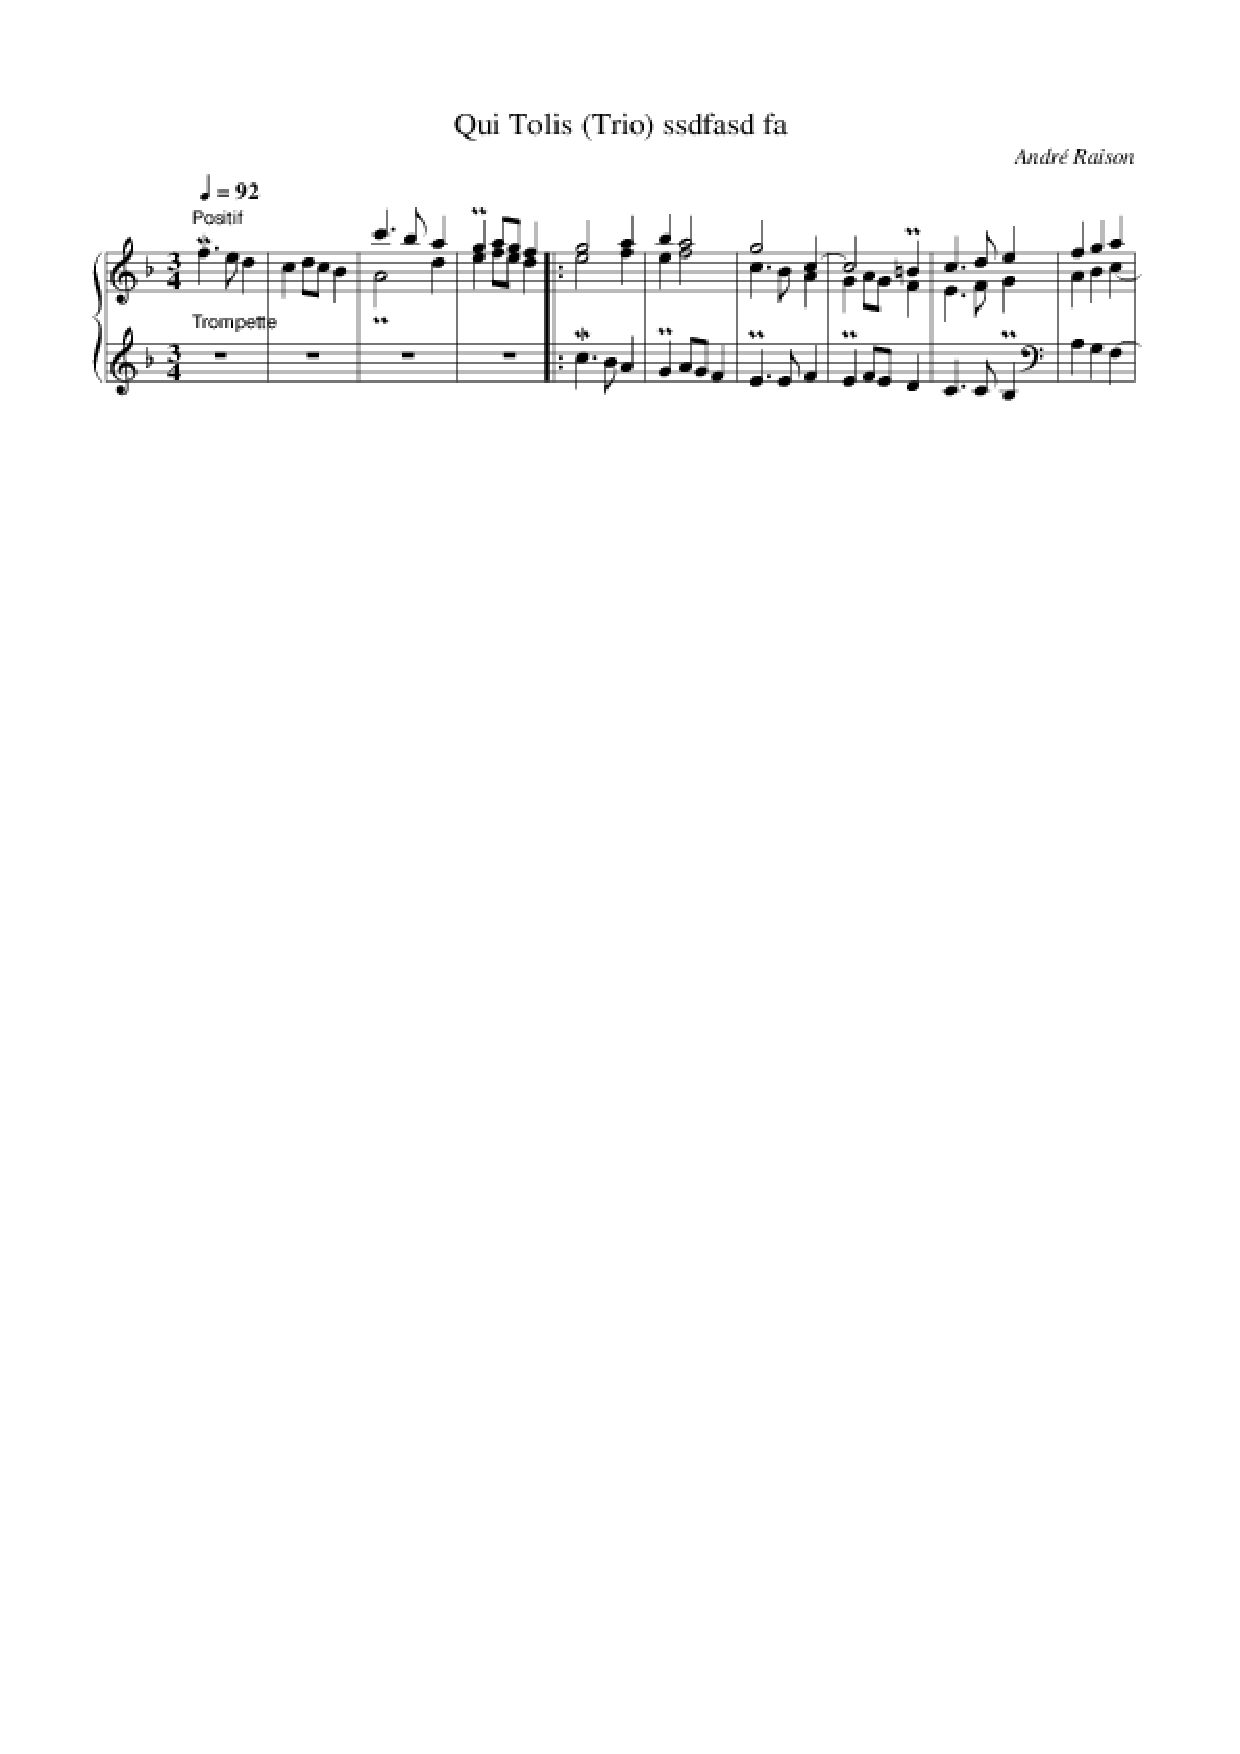
\includegraphics{../abc-images/60a0ca71335f79026e9bea175f1a09b2361f4748.pdf}

Use this

\begin{verbatim}
digraph G {Hello->World}
\end{verbatim}

to get

\begin{verbatim}
digraph G {Hello->World}
\end{verbatim}

with with Äüö

\begin{verbatim}
digraph G {Hello->World with Äüö}
\end{verbatim}

Use this

\begin{Shaded}
\begin{Highlighting}[]
\NormalTok{\textbackslash{}begin\{tikzpicture\}}

\NormalTok{\textbackslash{}def \textbackslash{}n \{5\}}
\NormalTok{\textbackslash{}def \textbackslash{}radius \{3cm\}}
\NormalTok{\textbackslash{}def \textbackslash{}margin \{8\} }\CommentTok{% margin in angles, depends on the radius}

\NormalTok{\textbackslash{}foreach \textbackslash{}s in \{1,...,\textbackslash{}n\}}
\NormalTok{\{}
  \NormalTok{\textbackslash{}node[draw, circle] at (\{360/\textbackslash{}n * (\textbackslash{}s - 1)\}:\textbackslash{}radius) \{$\textbackslash{}s$\};}
  \NormalTok{\textbackslash{}draw[->, >=latex] (\{360/\textbackslash{}n * (\textbackslash{}s - 1)+\textbackslash{}margin\}:\textbackslash{}radius) }
    \NormalTok{arc (\{360/\textbackslash{}n * (\textbackslash{}s - 1)+\textbackslash{}margin\}:\{360/\textbackslash{}n * (\textbackslash{}s)-\textbackslash{}margin\}:\textbackslash{}radius);}
\NormalTok{\}}
\NormalTok{\textbackslash{}end\{tikzpicture\}}
\end{Highlighting}
\end{Shaded}

to get

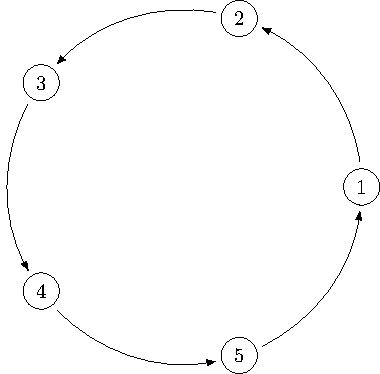
\includegraphics{../tikz-images/bb4ca6ef38e388bee5236368e2ae316cc8af1ed4.pdf}

\printbibliography

\end{document}
